\documentclass{acm_proc_article-sp}
\usepackage[utf8]{inputenc}
\usepackage{epstopdf}
\usepackage{times}
\usepackage{natbib}
\usepackage{amsmath}
\usepackage{dcolumn}
\usepackage{graphicx}
\usepackage{xspace}
\usepackage{color}
\usepackage{listings}
%\usepackage{amsmath, amsthm, amssymb, amsfonts}
%\usepackage{tabularx}
\usepackage{array}
%\usepackage{tabulary}%can use align in tables with line breaks
\usepackage{multirow}
\usepackage{rotating,makecell}
\usepackage{booktabs} %adds new commands toprule midrule and bottomrule for professionally looking tables

\usepackage[breaklinks=true, bookmarksopen=true,bookmarksnumbered=true]{hyperref}
\urlstyle{same}
% \usepackage{titling} % To modify the title
%\usepackage[hmargin=1.3in]{geometry}
% \setlength{\droptitle}{-5em}   % This is your set screw


\definecolor{Brown}{cmyk}{0,0.81,1,0.60}
\definecolor{OliveGreen}{cmyk}{0.64,0,0.95,0.40}
\definecolor{CadetBlue}{cmyk}{0.62,0.57,0.23,0}
\definecolor{lightlightgray}{gray}{0.9}

% listing styles
\lstset{
    numberbychapter=false,
    basicstyle=\ttfamily\footnotesize,
    numbers=none,
    captionpos=b,
    frame=single,
    breaklines=true,
    breakatwhitespace,
    columns=fullflexible,
    commentstyle=\itshape\color{OliveGreen},
    keywordstyle=\bfseries\color{CadetBlue}
}


\lstdefinestyle{SPARQL}{
  backgroundcolor=\color{lightlightgray}, % Choose background color
  morecomment=[l]{\#},
  morekeywords={SELECT, CONSTRUCT, FROM, WHERE, FILTER, GROUP BY, IN, AS,
    LIMIT,OFFSET,PREFIX,OPTIONAL,UNION,NOT,EXISTS,AVG,BIND,
    obs,foaf,rdf,skos,rdfs,ex,xsd,owl,skosxl,doap,void,dbo,earl,cex,qb}
 }

\lstdefinestyle{Turtle}{
  backgroundcolor=\color{lightlightgray}, % Choose background color
  morecomment=[l]{\#},
  morekeywords={@PREFIX,BASE,a,foaf, @prefix, rdf,
    obs,qb,cex,skos, skosxl, rdf, rdfs, ex, xsd, wr,
    wt,dc,lemon,doap,void,dbo,owl}
 }
    
\lstdefinestyle{Turtle}{numberblanklines=true, morekeywords={foaf, prefix, rdf,
    skos, skosxl, rdfs, ex, xsd, wr, wt, dc, lemon, doap, doap,void, dbo, owl,
    @prefix}}


%\usepackage{textcomp}
\lstdefinestyle{XML}
{
  morestring=[b]",
  morestring=[s]{>}{<},
  morecomment=[s]{<?}{?>},
  stringstyle=\color{black},
  identifierstyle=\color{darkblue},
  keywordstyle=\color{cyan},
  morekeywords={xmlns,version,type}% list your attributes here
}

\sloppy

%%%%%%%%%%% Put your definitions here


%%%%%%%%%%% End of definitions

\newcommand{\TODO}[1]{{\color{red}{\textbf{TODO: {#1}}\xspace}}}
\newcommand{\todo}[1]{{\TODO{{#1}}}}

\newcommand{\CONSIDER}[1]{{\color{blue}{\textbf{CONSIDER: {#1}}\xspace}}}
   
\newcommand{\desc}{\noindent\emph{Description:}}

\newcommand{\footnoteUrl}[1]{\footnote{\url{#1}}}

\newcolumntype{d}[1]{D{.}{.}{#1}}


\begin{document}

\title{Representing verifiable statistical index computations as linked data}

\numberofauthors{3} 
\author{
\alignauthor
Jose Emilio Labra Gayo\\
       \affaddr{University of Oviedo}\\
       \affaddr{Dept. of Computer Science}\\
       \affaddr{C/Calvo Sotelo, S/N}\\
       \email{labra@uniovi.es}
\alignauthor
Hania Farham\\
       \affaddr{The Web Foundation}\\
       \email{hania@webfoundation.org}
\alignauthor
Juan Castro Fernández\\
       \affaddr{WESO Research Group} \\
       \affaddr{University of Oviedo}\\
       \affaddr{C/Calvo Sotelo, S/N}\\
       \email{juan.castro@weso.es}
}

\maketitle
\begin{abstract}

In this paper we describe the development of the Web Index linked data portal that represents statistical index data and computations. 

 The Web Index is a multi-dimensional measure of the World Wide Web’s contribution to development and human rights globally. It covers 81 countries and incorporates indicators that assess several areas like universal access; freedom and openness; relevant content; and empowerment.

In order to empower the Web Index transparency, one internal requirement was that every published data could be externally verified. 
The verification could be that it was just raw data obtained from an external source, in which case, the system must provide a link to the data source or that the value has been internally computed, 
 in which case, the system provides links to those values.
The resulting portal contains data that can be tracked to its sources so an external agent
can validate the whole index computation process.

We describe the different aspects on the development of the WebIndex data portal, which also offers new linked data visualization tools. 

Although in this paper we concentrate on the Web Index development, 
we consider that this approach can be generalized to other projects which involve 
 the publication of externally verifiable statistical computations.
\end{abstract}

% A category with the (minimum) three required fields
\category{H.2.8}{Database Applications}{Statistical databases}
%A category including the fourth, optional field follows...
\category{H.3.5}{Online Information Services}{Web-based services}

\terms{Theory}

\keywords{Linked data, Statistics, Computations, RDF} 

\section{Introduction}

The creation and use of quantitative indexes is a widely 
accepted practice that has been applied to numerous domains like economics and
Bibliometrics (Impact factor), 
research and academic performance (H-Index or Shanghai rankings), 
 cloud computing (Global Cloud Index, by CISCO), 
etc.

We consider that those indexes could benefit from a 
 Linked Data approach where the rankings could be seen, tracked and 
 verified by their users.

We participated in the Web Index project
(\url{http://thewebindex.org}), which created an index to measure 
 the Web impact in different countries.

The 2012 version offered a data
portal\footnoteUrl{http://data.webfoundation.org} whose data was obtained 
by transforming raw observations and precomputed values 
from Excel sheets to RDF~\cite{Alvarez13}. 

In the 2013 version of that data portal, we are working on 
both validating and computing observations to automatically generate
the index from raw data.

We have defined a generic vocabulary 
of computational index structures which could be applied to compute and validate any other kind of
index and can be seen as an instance of the RDF Data Cube
vocabulary~\cite{Cube}.
The validation process employs SPARQL~\cite{SPARQL11} queries to model the 
 different integrity constraints and computation steps in a declarative way.


%At this moment, we have a running example and a validator which 
% reads and executes the SPARQL queries. 
% Source code and some examples are available
% at~\url{https://github.com/weso/computex}. 
% Although our prototype validator has been implemented in Scala, 
% our approach is independent of any programming language 
% as far as it can load and execute SPARQL 1.1 queries.

 Along the paper we will use Turtle and SPARQL notation and assume that the
namespaces have been declared using the most common prefixes found in
\url{http://prefix.cc}.

\section{WebIndex workflow}

\begin{figure*}[h]
\label{Fig:WebIndexWorkFlow}
\begin{center}
  \makebox[\textwidth]{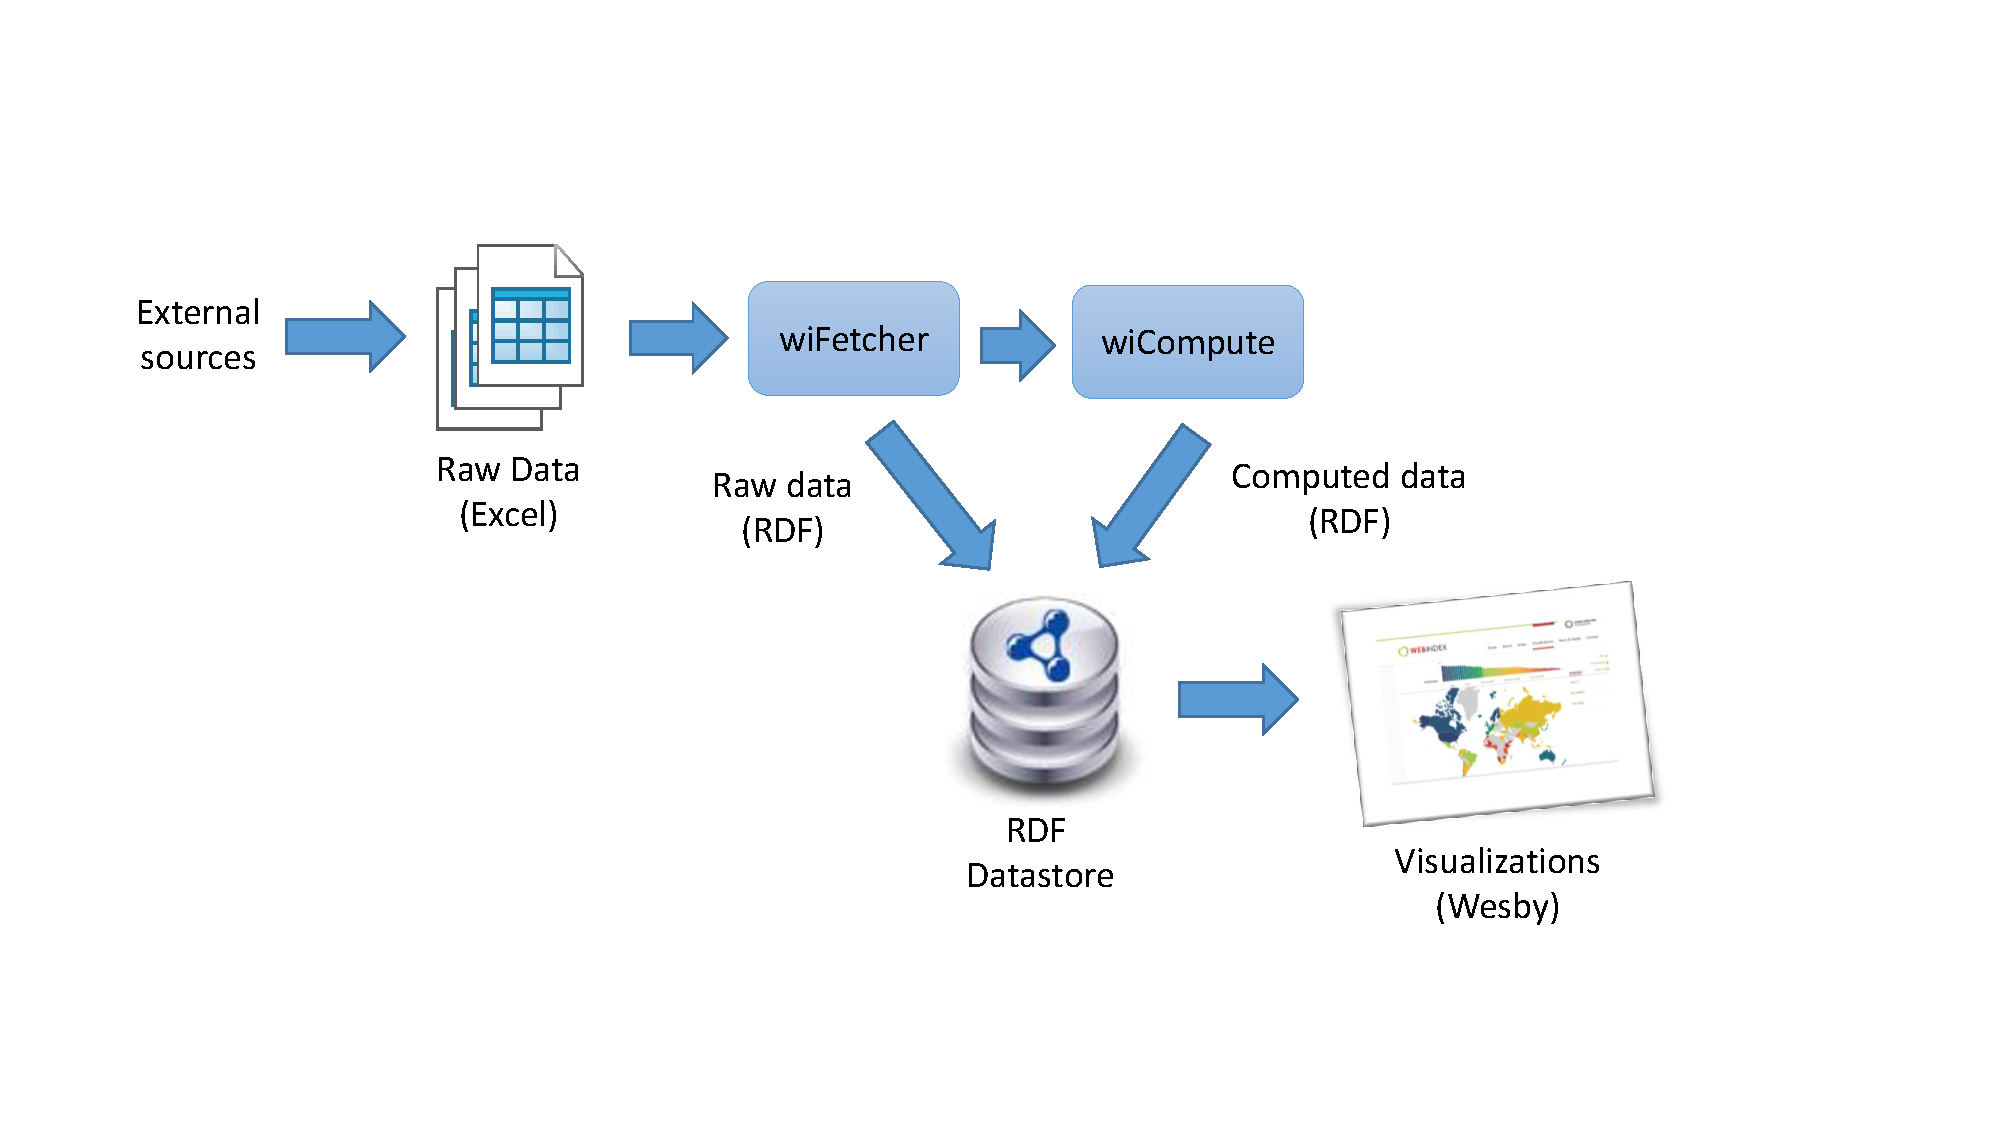
\includegraphics[width=\textwidth]{WebIndexWorkFlow}}
\end{center}
\caption{Web Index data portal WorkFlow}
\end{figure*}

\section{WebIndex computation model}

Our data model consists of a list of observations which can be raw observations
obtained from an external source or computed observations derived from other
observations. An example observation can be:

\begin{lstlisting}[style=SPARQL]
obs:obsM23 a qb:Observation ;
 cex:computation [ a cex:Z-Score ; 
      cex:observation obs:obsA23 ; cex:slice slice:sliceA09 ; ] ;
 cex:value 0.56 ;
 cex:md5-checksum "2917835203..." ;
 cex:indicator indicator:A ;
 cex:concept country:ESP ;
 qb:dataSet dataset:A-Normalized ;
 # ... other declarations omitted for brevity
\end{lstlisting}

Where we declare that \lstinline|obs:obsM23| is an observation
 whose value is \lstinline|0.56| that has been obtained as the Z-Score
 of the observation \lstinline|obs:A23| using the slice
 \lstinline|slice:sliceA09|. The observations refers to indicator
 \lstinline|indicator:A|, to the concept \lstinline|country:ESP| and to the
 dataset \lstinline|dataset:A-Normalized|.
 
For each observation, we also add a value for 
\lstinline|cex:md5-checksum| which is obtained as a combination of the 
different values of the observation and allows a user to verify the
values asserted to that observation.


\section{Computex vocabulary}

The \emph{Computex} vocabulary is available
at~\url{http://purl.org/weso/computex}. It defines terms related to the
computation of statistical index data and is compatible with RDF Data Cube
vocabulary. Some terms defined in the vocabulary are:

\begin{itemize}
\item\textbf{\lstinline|cex:Concept|} represents the entities that we are
indexing.
In the case of the Web Index project, the concepts are the different countries.
In other applications it could be Universities, journals, services, etc.

\item\textbf{\lstinline|cex:Indicator|}. A dimension whose values add
information to the Index.
Indicators can be simple dimensions, for example: the mobile phone
suscriptions per 100 population, or can be composed from other
indicators. 

\item\textbf{\lstinline|qb:Observation|}. This is the same term as in the 
RDF Data Cube vocabulary. It contains values for the
properties: \lstinline|cex:value|, \lstinline|cex:indicator| 
and \lstinline|cex:concept|, etc. 
The value of a \lstinline|qb:Observation| can be a Raw value
   obtained from an external source or a computed value obtained from other
   observations.

\item\textbf{\lstinline|cex:Computation|}. We have declared the main computation
types that we needed for the WebIndex project, which have been summarized in
Table~\ref{table:computations}. That list of computation types is non-exhaustive
and can be further extended in the future. 

\item\textbf{\lstinline|cex:WeightSchema|} a weight schema for a list of
indicators. It consists of a weight associated for each indicator which can be
used to compute an aggregated observation.

\end{itemize}

\begin{table*}[t]
\label{table:computations}
\begin{center}
\begin{tabular}{ p{0.2\textwidth} p{0.5\textwidth} p{0.3\textwidth}}
\toprule
Computation & Description & Properties \\
\hline
Raw			& No computation. Raw value obtained from external source.
			&  \\
Mean	    & Mean of a set of observations 
			& \lstinline|cex:observation| \newline 
			  \lstinline|cex:slice| \\
Increment	& Increment an observation by a given amount 
			& \lstinline|cex:observation| \newline 
			  \lstinline|cex:amount|  \\
Copy		& A copy of another observation 
			& \lstinline|cex:observation| \\
Z-score		& A normalization of an observation using the values from a Slice. 
			& \lstinline|cex:observation| \newline 
			  \lstinline|cex:slice| \\
Ranking		& Position in the ranking of a slice of observations. 
			& \lstinline|cex:observation| \newline 
			  \lstinline|cex:slice| \\
AverageGrowth & Expected average growth of N observations
			  & \lstinline|cex:observations| \\
WeightedMean & Weighted mean of an observation
			& \lstinline|cex:observation| \newline
			  \lstinline|cex:slice|       \newline
			  \lstinline|cex:weightSchema| \\
\bottomrule\\
\end{tabular}
\caption{Some types of statistical computations}
\end{center}
\end{table*}

\section{Validation approach}

The validation approach employed in the 2012 WebIndex project was based on
 resource templates similar to the OSLC resource
 shapes\footnoteUrl{http://www.w3.org/2012/12/rdf-val/SOTA} and
 the MD5 checksum field. 
 Apart from that, we did not verify that the precomputed values imported from
 the Excel sheets really match the value that could be obtained by 
 following the declared computation process.

The new validation approach proposed in the paper goes a step forward. 
The goal is not only to check that a resource contains
 a given set of fields and values, but also that those values really match
 the values that can be obtained by following the declared computations.
 
The proposed approach has been inspired by the integrity
constraint specification proposed by the RDF Data Cube vocabulary 
which employs a set of SPARQL
 \lstinline|ASK| queries to check the integrity of RDF Data Cube data. 
 Although \lstinline|ASK| queries provide a good means to check integrity, in
 practice their boolean nature does not offer too much help when a 
 dataset does not accomplish with the data model.

 We decided to use \lstinline|CONSTRUCT| queries which, in case of error, 
  contain an error message and a list of error parameters that can help to spot
  the problematic data.

 We transformed the \lstinline|ASK| queries defined in the RDF Data Cube
 specification to \lstinline|CONSTRUCT| queries. For example, the
 query to validate the RDF Data Cube integrity constraint 4 (IC-4) is:
 
\begin{lstlisting}[style=SPARQL]
CONSTRUCT {
 [ a cex:Error ; cex:errorParam [cex:name "dim"; cex:value ?dim ] ;
   cex:msg "Every Dimension must have a declared range" . ]
} WHERE { ?dim a qb:DimensionProperty .
  FILTER NOT EXISTS { ?dim rdfs:range [] }
}
\end{lstlisting}
 
In order to make our error messages compatible with EARL~\cite{EARL}, we have
 defined \lstinline|cex:Error| as a subclass of \lstinline|earl:TestResult| and 
 declared it to have the value \lstinline|earl:failed| for the property
 \lstinline|earl:outcome|.
 
We have also created our own set of SPARQL \lstinline|CONSTRUCT| queries to
validate the \emph{Computex} vocabulary terms, specially the computation of index data.
For example, the following query validates that every observation 
  has at most one value.
 
\begin{lstlisting}[style=SPARQL]
CONSTRUCT {
 [ a cex:Error ; cex:errorParam  # ... omitted 
    cex:msg "Observation has two different values" . ]
} WHERE { ?obs a qb:Observation . 
 ?obs cex:value ?value1 . ?obs cex:value ?value2 .
 FILTER ( ?value1 != ?value2  )
}
\end{lstlisting}

Using this approach, it is possible to define more expressive validations.
For example, we are able to validate that an observation has been obtained as
the mean of other observations. 

\begin{lstlisting}[style=SPARQL]
CONSTRUCT {
 [ a cex:Error ; cex:errorParam # ...omitted 
   cex:msg "Mean value does not match" ] . 
} WHERE { 
    ?obs a qb:Observation ;
         cex:computation ?comp ;
         cex:value ?val .
  ?comp a cex:Mean .
  { SELECT (AVG(?value) as ?mean) ?comp WHERE {
     ?comp cex:observation ?obs1 .
	 ?obs1 cex:value ?value ;
  } GROUP BY ?comp } 
 FILTER( abs(?mean - ?val) > 0.0001)
}
\end{lstlisting}

\section{Expressivity limits of SPARQL queries}

Validating statistical computations using SPARQL queries offered 
 a good exercise to check SPARQL expressivity. Although we were able 
 to express most of the computation types, some of them had to employ functions
 that are not part of SPARQL 1.1 or had to be defined in a limited way. 
 In this section we review some of the challenges that we found.

\begin{itemize} 

\item The Z-score of a value $x_i$ is defined as $\frac{x - \bar{x}}{\sigma}$
where $\bar{x}$ is the mean and $\sigma=\sqrt{\frac{\sum_{i=1}^{N}(\bar{x}-x_i)^2}{N -
1}}$ is the standard deviation. To validate that computation using SPARQL
queries, it is necessary to employ the \lstinline|sqrt| function. 
This function is not available in SPARQL 1.1 although some implementations 
 like Jena
 ARQ\footnoteUrl{http://jena.apache.org/documentation/query/library-function.html} 
 provide it.

\item In order to validate the ranking of an observation (in which position it
appears in a list of observations), we have found two approaches. One is to
check all the observations that are below the value of that observation. 
This approach requires checking the value of each observation against all the
other values. The other approach is to use a subquery that groups all the
observations ordered by their value using the \lstinline|GROUP_CONCAT|. 
However, SPARQL does not offer a function to calculate the position
of a substring in a string\footnote{This function is called \lstinline|strpos| in PHP or \lstinline|indexOf| in Java}, 
so we divided the length of the substring before the concept's 
name by the length of the concept's name. 
This approach is more efficient but only works when all the names have
the same length.

\item Given a list of values $x_1,x_2\ldots{}x_n$ the expected value
$x_{n+1}$ can be extrapolated using the forward average growth formula: 
$x_n\times{\frac{\frac{x_{n}}{x_{n-1}}+\ldots{}+\frac{x_{2}}{x_1}}{n-1}}$. 
Accessing RDF collections in SPARQL 1.1 requires property paths 
and offers limited expressivity. In this particular case 
the query can be expressed 
as\footnote{This query was suggested by Joshua Taylor.}:

\begin{lstlisting}[style=SPARQL]
CONSTRUCT {
  # ... omitted for brevity
} WHERE { 
  ?obs cex:computation [a cex:AverageGrowth; cex:observations ?ls] ;
  cex:value ?val .
  ?ls rdf:first [cex:value ?v1 ] .
  { SELECT ( SUM(?v_n / ?v_n1)/COUNT(*) as ?meanGrowth) WHERE {
      ?ls rdf:rest* [ rdf:first [ cex:value ?v_n ] ; 
                      rdf:rest  [ rdf:first [ cex:value ?v_n1 ]]] .
  }} 
 FILTER (abs(?meanGrowth * ?v1 - ?val) > 0.001) }
\end{lstlisting}

\end{itemize}

\section{Visualizing the Web Index}

\section{Related work}

\TODO{Validating RDF}
\TODO{Statistical vocabularies}
\TODO{Vocabularies to represent computations}

\section{Conclusions}

Using SPARQL queries to validate and compute index data seems a promising use
case for linked data applications. 
Although we have successfully employed this approach to validate most of the
statistical computations we needed for the WebIndex project, we have found some
limitations in current SPARQL 1.1 expressivity with regards to built-in
functions on maths, strings and RDF Collections.

We consider that our approach may be of interest to the RDF Validation 
 workshop in 2 ways: firstly as a practical approach to validate RDF data
 which poses some expressivity challenges, and secondly, as a 
 use case with real data than can act as a benchmark to compare different
 validation strategies.

Our future work is to automate the declarative computation of index data
 from the raw observations and to check the performance using
 the Web Index data. 
We are also studying the feasibility of this approach 
 for online calculation of index scores and rankings. 
% \TODO{Visualization of computed values?}

\bibliographystyle{abbrv}
\bibliography{computex}

\end{document}
